%%%%%%%%%%%%%%%%%%%%%%%%%%%%%%%%%%%%%%%%%
% Masters/Doctoral Thesis 
% LaTeX Template
% Version 2.5 (27/8/17)
%
% This template was downloaded from:
% http://www.LaTeXTemplates.com
%
% Version 2.x major modifications by:
% Vel (vel@latextemplates.com)
%
% This template is based on a template by:
% Steve Gunn (http://users.ecs.soton.ac.uk/srg/softwaretools/document/templates/)
% Sunil Patel (http://www.sunilpatel.co.uk/thesis-template/)
%
% Template license:
% CC BY-NC-SA 3.0 (http://creativecommons.org/licenses/by-nc-sa/3.0/)
%
%%%%%%%%%%%%%%%%%%%%%%%%%%%%%%%%%%%%%%%%%

%----------------------------------------------------------------------------------------
%	PACKAGES AND OTHER DOCUMENT CONFIGURATIONS
%----------------------------------------------------------------------------------------

\documentclass[
12pt, % The default document font size, options: 10pt, 11pt, 12pt
%oneside, % Two side (alternating margins) for binding by default, uncomment to switch to one side a activer si on veut qu'il n'y ait pas de décalage de la marge une page sur deux et que la pagination soit une fois à droite et une fois à gauche (c'est le cas où l'on imprime recto-verso).
french, % ngerman for German
singlespacing, % Single line spacing, alternatives: onehalfspacing or doublespacing
%draft, % Uncomment to enable draft mode (no pictures, no links, overfull hboxes indicated)
%nolistspacing, % If the document is onehalfspacing or doublespacing, uncomment this to set spacing in lists to single
%liststotoc, % Uncomment to add the list of figures/tables/etc to the table of contents
%toctotoc, % Uncomment to add the main table of contents to the table of contents
%parskip, % Uncomment to add space between paragraphs
%nohyperref, % Uncomment to not load the hyperref package
headsepline, % Uncomment to get a line under the header
%chapterinoneline, % Uncomment to place the chapter title next to the number on one line
%consistentlayout, % Uncomment to change the layout of the declaration, abstract and acknowledgements pages to match the default layout
]{MastersDoctoralThesis} % The class file specifying the document structure

% \usepackage[frenchb]{babel}
\usepackage[utf8]{inputenc} % Required for inputting international characters
\usepackage[T1]{fontenc} % Output font encoding for international characters
\usepackage{mathpazo} % Use the Palatino font by default
\usepackage[
backend=bibtex]{biblatex} % Use the bibtex backend with the authoryear citation style (which resembles APA)

\addbibresource{bibliography/bibliography.bib} % The filename of the bibliography

\usepackage[autostyle=true]{csquotes} % Required to generate language-dependent quotes in the bibliography

\usepackage{algorithm}
\usepackage{algpseudocode}
%----------------------------------------------------------------------------------------

% Define some commands to keep the formatting separated from the content 
\newcommand{\keyword}[1]{\textbf{#1}}
\newcommand{\tabhead}[1]{\textbf{#1}}
\newcommand{\code}[1]{\texttt{#1}}
\newcommand{\file}[1]{\texttt{\bfseries#1}}
\newcommand{\option}[1]{\texttt{\itshape#1}}

%----------------------------------------------------------------------------------------

%----------------------------------------------------------------------------------------
%	MARGIN SETTINGS
%----------------------------------------------------------------------------------------

\geometry{
	paper=a4paper, % Chrvisange to letterpaper for US letter
	inner=2.5cm, % Inner margin
	outer=3.8cm, % Outer margin
	bindingoffset=.5cm, % Binding offset
	top=1.5cm, % Top margin
	bottom=1.5cm, % Bottom margin
	%showframe, % Uncomment to show how the type block is set on the page
}

%----------------------------------------------------------------------------------------
%	THESIS INFORMATION
%----------------------------------------------------------------------------------------
\thesistitle{Stratégies de recherche et application au test logiciel} % Your thesis title, this is used in the title and abstract, print it elsewhere with \ttitle
\supervisor{MCF. Emmanuel \textsc{Hyon}} % Your supervisor's name, this is used in the title page, print it elsewhere with \supname
\examiner{} % Your examiner's name, this is not currently used anywhere in the template, print it elsewhere with \examname
\author{Valentin \textsc{Bouquet}} % Your name, this is used in the title page and abstract, print it elsewhere with \authorname
\addresses{valentin-bouquet@hotmail.fr} % Your address, this is not currently used anywhere in the template, print it elsewhere with \addressname

\keywords{heuristiques, exploration de chemins, test logiciel, génie logiciel, exécution symbolique, monte carlo tree search} % Keywords for your thesis, this is not currently used anywhere in the template, print it elsewhere with \keywordnames
\university{\href{http://www.parisnanterre.fr/}{Université Paris Nanterre}} % Your university's name and URL, this is used in the title page and abstract, print it elsewhere with \univname
\department{\href{https://www.parisnanterre.fr/organisation/departement-de-mathematiques-et-informatique-343280.kjsp}{Département de mathématiques et informatique}} % Your department's name and URL, this is used in the title page and abstract, print it elsewhere with \deptname

\AtBeginDocument{
\hypersetup{pdftitle=\ttitle} % Set the PDF's title to your title
\hypersetup{pdfauthor=\authorname} % Set the PDF's author to your name
\hypersetup{pdfkeywords=\keywordnames} % Set the PDF's keywords to your keywords
}

\begin{document}
% \let\cleardoublepage\clearpage % A activer pour supprimer les pages blanches entre chapitres, table des matières, remerciements, etc.

\frontmatter % Use roman page numbering style (i, ii, iii, iv...) for the pre-content pages

\pagestyle{plain} % Default to the plain heading style until the thesis style is called for the body content

%----------------------------------------------------------------------------------------
%	TITLE PAGE
%----------------------------------------------------------------------------------------

\begin{titlepage}
\begin{center}

\vspace*{.06\textheight}
{\scshape\LARGE \univname \par}\vspace{1.5cm} % University name
\textsc{\Large Mémoire de fin d'études\\-\\MIAGE}\\[0.5cm] % Thesis type

\HRule \\[0.4cm] % Horizontal line
{\huge \bfseries \ttitle\par}\vspace{0.4cm} % Thesis title
\HRule \\[1.5cm] % Horizontal line
 
\begin{minipage}[t]{0.4\textwidth}
\begin{flushleft} \large
\emph{Auteur:}\\
\href{http://www.github.com/vbouquet}{\authorname} % Author name - remove the \href bracket to remove the link
\end{flushleft}
\end{minipage}
\begin{minipage}[t]{0.4\textwidth}
\begin{flushright} \large
\emph{Tuteur:} \\
\href{https://www.lip6.fr/actualite/personnes-fiche.php?ident=P216}{\supname} % Supervisor name - remove the \href bracket to remove the link  
\end{flushright}
\end{minipage}\\[3cm]
 
% \vfill

% \vfill

{\large \today}\\[4cm] % Date

\includegraphics[scale=0.75]{figures/logo-paris-nanterre.jpg} % University/department logo - uncomment to place it
 
\vfill
\end{center}
\end{titlepage}

%----------------------------------------------------------------------------------------
%	QUOTATION PAGE
%----------------------------------------------------------------------------------------

% \vspace*{0.2\textheight}

% \noindent\enquote{\itshape }\bigbreak

% \hfill Valentin Bouquet

%----------------------------------------------------------------------------------------
%	Résumé (abstract)
%----------------------------------------------------------------------------------------

\newenvironment{abstract}%
{\cleardoublepage\thispagestyle{empty}\null\vfill\begin{center}%
\bfseries\abstractname\end{center}}%
{\vfill\null}

\begin{abstract}

«Tester revient à confronter par des moyens statiques (analyse de code, revue, etc.) ou par des moyens dynamiques (exécution avec des valeurs particulières) les spécifications du logiciel, c’est à dire ce qu’il doit faire et éventuellement sous quelles contraintes (temps, utilisation de la mémoire, etc.), à sa réalisation, c’est à dire de quelle façon il répond au besoin exprimé en enchainant différentes actions élémentaires.»\cite{jfpp-test}

La génération automatique de tests est un domaine déjà bien développé qui permet aujourd'hui grâce à différentes analyse à partir du code comme celle de l'arbre syntaxique abstrait, du graphe de flot de contrôle (CFG) et d'application de méthodes comme l'exécution symbolique, concolique ou de model-checking d'extraire des propriétés parfois abstraites du code pour identifier des valeurs de tests pertinentes pour s'assurer de la qualité du programme.

Ces approches sont malheureusement limitées de par la complexité grandissante des programmes à tester qui confronte ces méthodes à l'explosion du nombre de chemins, du nombre d'états ou de contraintes possibles. Pour représenter ces états et chemins, ces méthodes repose sur des modèles d'arbres qui ne peuvent être parcourus en intégralité à cause de leur taille. Les algorithmes de parcours actuellement utilisés repose souvent sur des stratégies simples comme le parcours en profondeur qui est connu pour être particulièrement couteux.

Ces dernières années, grâce la maturation des recherches sur les différentes stratégies et heuristiques de parcours de graphe (et notamment celles avec apprentissage) et des applications récentes sur des problèmes concrets comme l'ordinateur \textit{AlphaGo} qui grâce à une implémentation de l'heuristique du Monte Carlo Tree Search a réussi à battre le champion du monde actuel, ces méthodes ce sont popularisées.

Dans ce mémoire, nous présentons la notion d'heuristique, les différentes modélisations possibles, les algorithmes de parcours populaires, des heuristiques d'apprentissage et plus particulièrement les heuristiques Monte Carlo Tree Search (MCTS) ainsi que des applications au test logiciel. 
Enfin nous regardons si il serait possible d'appliquer des heuristiques de recherches (intelligentes) pour la génération de tests et plus particulièrement à des fins de faciliter l'apprentissage de la programmation.\\

\textbf{Mots clés:} \keywordnames
%Le test d'application est une part importante du cycle de développement d'une application. Le coût des tests occupe entre 30\% et 50\% du développement.
%La génération de cas de tests est une des tâches les plus laborieuses lors du test d'application.
%Une grande partie des limitations de l'analyse logiciel vient de la complexité pour établir tous les cas.
...
% Facilité la maintenance de la qualité logicielle au cours des évolutions.


\end{abstract}

%----------------------------------------------------------------------------------------
%	Remeciements
%----------------------------------------------------------------------------------------
\ohead*{} % Numéro de page en haut
\ofoot*{\pagemark} % Numéro de page en bas
\begin{acknowledgements}

%TODO
Cette année est l'aboutissement de 5 années d'études universitaires et je tiens donc à saluer tous les enseignants et chercheurs que j'ai pu côtoyer durant toutes ces années ainsi que tous les étudiants des formations classiques et en apprentissage, de la licence au master de la \textit{MIASH} et de la \textit{MIAGE} de Paris-Nanterre.\\

Je pense aussi aux opportunités qui se sont présentées à moi afin de poursuivre mes études sereinement dans le supérieure. Il ne fait aucun doute que le climat universitaire français est généreux et que sans lui il m'aurait été impossible de continuer comme je l'ai fait. J'espère que les générations futures seront tout aussi à mène d'en bénéficier et de savourer cette chance. En espérant que les entraves à ce système s'essoufflent et laisse place à un avenir plus prometteur.\\

Je remercie Emmanuel Hyon pour son encadrement, son écoute et pour sa bienveillance envers ses étudiants ainsi que pour ses conseils qu'il a su me prodiguer, y compris pour la rédaction de ce mémoire.\\

Je remercie particulièrement François Delbot et Jean-François Pradat-Peyre pour tout le soutien qu'ils m'ont porté et de m'avoir permis de travailler dans d'excellentes conditions. Je les remercie vivement pour tout les conseils, avis et discussions qu'ils m'ont apportés qui m'ont ouvert vers de nouvelles horizons.
Sans leurs soutiens, je n'aurais jamais une seconde pu imaginer poursuivre un travail de recherche. J'espère que ces récents espoirs seront trouver satisfaction.

\end{acknowledgements}


%----------------------------------------------------------------------------------------
%	LIST OF CONTENTS/FIGURES/TABLES PAGES
%----------------------------------------------------------------------------------------

\tableofcontents % Prints the main table of contents

% \listoffigures % Prints the list of figures

% \listoftables % Prints the list of tables

%----------------------------------------------------------------------------------------
%	ABBREVIATIONS
%----------------------------------------------------------------------------------------

% \begin{abbreviations}{ll} % Include a list of abbreviations (a table of two columns)

% \textbf{LAH} & \textbf{L}ist \textbf{A}bbreviations \textbf{H}ere\\
% \textbf{WSF} & \textbf{W}hat (it) \textbf{S}tands \textbf{F}or\\

% \end{abbreviations}

%----------------------------------------------------------------------------------------
%	THESIS CONTENT - CHAPTERS
%----------------------------------------------------------------------------------------

\mainmatter % Begin numeric (1,2,3...) page numbering
\pagestyle{thesis} % Return the page headers back to the "thesis" style

% Include the chapters of the thesis as separate files from the Chapters folder
% Uncomment the lines as you write the chapters

\chapter*{Introduction}
\addchaptertocentry{Introduction}
%TODO 
«Tester revient à confronter par des moyens statiques (analyse de code, revue, etc.) ou par des moyens dynamiques (exécution avec des valeurs particulières) les spécifications du logiciel, c’est à dire ce qu’il doit faire et éventuellement sous quelles contraintes (temps, utilisation de la mémoire, etc.), à sa réalisation, c’est à dire de quelle façon il répond au besoin exprimé en enchainant différentes actions élémentaires.»\cite{jfpp-test}\cite{judea-pearl-heuristics}\cite{MCTS-methods-survey}\cite{MTCS-symbolic-execution-path-exploration}\cite{MTCS-program-synthesis}\cite{MTCS-symbolic-execution-less-path}\cite{testing-and-machine-learning}

La génération automatique de tests est un domaine déjà bien développé qui permet aujourd'hui grâce à différentes analyse à partir du code comme celle de l'arbre syntaxique abstrait, du graphe de flot de contrôle (CFG) et d'application de méthodes comme l'exécution symbolique, concolique ou de model-checking d'extraire des propriétés parfois abstraites du code pour identifier des valeurs de tests pertinentes pour s'assurer de la qualité du programme\cite{EFSM}  .

Ces approches sont malheureusement limitées de par la complexité grandissante des programmes à tester qui confronte ces méthodes à l'explosion du nombre de chemins, du nombre d'états ou de contraintes possibles. Pour représenter ces états et chemins, ces méthodes repose sur des modèles d'arbres qui ne peuvent être parcourus en intégralité à cause de leur taille. Les algorithmes de parcours actuellement utilisés repose souvent sur des stratégies simples comme le parcours en profondeur qui est connu pour être particulièrement couteux.

Ces dernières années, grâce la maturation des recherches sur les différentes stratégies et heuristiques de parcours de graphe (et notamment celles avec apprentissage) et des applications récentes sur des problèmes concrets comme l'ordinateur \textit{AlphaGo} qui grâce à une implémentation de l'heuristique du Monte Carlo Tree Search a réussi à battre le champion du monde actuel, ces méthodes ce sont popularisées.

Dans ce mémoire, nous présentons la notion d'heuristique, les différentes modélisations possibles, les algorithmes de parcours populaires, des heuristiques d'apprentissage et plus particulièrement les heuristiques Monte Carlo Tree Search (MCTS) ainsi que des applications au test logiciel. 
Enfin nous regardons si il serait possible d'appliquer des heuristiques de recherches (intelligentes) pour la génération de tests et plus particulièrement à des fins de faciliter l'apprentissage de la programmation\cite{symbolic-execution-machine-learning}.\\

Ces dernières années des méthodes d'intelligence artificielles ont été appliqués dans de nombreux domaines, c'est le cas par exemple de l'ordinateur X qui a battu le joueur Y au jeu de GO grâce à un algorithme reposant sur la famille des Monte Carlo Tree Search, méthode de recherche basé sur l'apprentissage\cite{shadow}.

Émergence de solutions pratiques\cite{ART} car la recherche est disponible (30ans de recherche d'IA) et que l'aire de big data ont permis l'émergence de cas d'applications concrets.

Intérêt: utiliser les méthodes de recherches arborescentes informées permettant de trouver des solutions à un problème donné à forte combinatoire et ceci en un temps raisonnable.

Le test et la vérification logiciel est un domaine très important pour X, Y et Z.
La vérification de logiciel et la génération de tests est souvent limité à cause de la complexité des programmes et des ressources limités des ordinateurs actuels.

%TODO A supprimer (pour voir les citations en fait)
%----------------------------------------------------------------------------------------
%	CHAPITRE 1
%----------------------------------------------------------------------------------------
\chapter{Test logiciel et automatisation} % Nom du premier chapitre

\label{Chapter1} % For referencing the chapter elsewhere, use \ref{Chapter1} 


%----------------------------------------------------------------------------------------
%	SECTION 1
%----------------------------------------------------------------------------------------
\section{Introduction}

%TODO INTRODUCTION
« Tester revient à confronter par des moyens statiques (analyse de code, revue, etc.) ou par des moyens dynamiques (exécution avec des valeurs particulières) les spécifications du logiciel, c’est à dire ce qu’il doit faire et éventuellement sous quelles contraintes (temps, utilisation de la mémoire, etc.), à sa réalisation, c’est à dire de quelle façon il répond au besoin exprimé en enchainant différentes actions élémentaires. »\cite{jfpp-test}

Le test logiciel est une part importante du cycle de développement d'une application et devient vite indispensable pour pérenniser les projets puisqu'elle permet à la fois de s'assurer du comportement d'un logiciel mais aussi de faciliter la maintenance en écartant tous cas de régression lors de l'ajout de nouvelles fonctionnalités ou de simples patchs correctifs.

L'importance de cette activité dépend fortement du domaine de l'application.
Par exemple quand la sécurité des données d'une société, d'un chef d'état ou des vies humaines peuvent être impactés par l'exécution d'un programme comme c'est le cas dans les logiciels embarqués en aéronautique, elle prend une place prépondérante et on ira jusqu'à utiliser des techniques de vérification pour s'assurer à un taux proche de 100\% que l'exécution du logiciel correspond aux spécifications définies. 
Une telle assurance est parfois fondamentale puisque une erreur lors de l'écriture du logiciel peut causer un \textit{bug} majeur et être particulièrement couteuse. Un des cas les plus célèbres est celui-ci associé au programme du décollage de la fusée Ariane 5\cite{ariane5} qui eu pour cause l'explosion de celle ci en plein vol après seulement quelques secondes de décollage. Erreur causée par le plantage du système de guidage inertiel principal à cause d'un simple dépassement d'entier, qui aurait donc pu être corrigé en testant les bornes maximales des entiers.

Cette activité à tout de même de nombreux inconvénients puisqu'elle demande du temps pour être réalisée correctement mais aussi une certaine expertise et est plutôt exigeante intellectuellement. Il ne s'agit pas de tester le programme au hasard en espérant trouver des erreurs mais il faut parfois penser plus loin que le comportement général du programme et donc analyser aussi le comportement des fonctions, des composants et de leurs intégrations avec d'autres logiciels ou d'autres environnements.

Le test logiciel est donc couteux et on lui attribue souvent à lui seul 50\% à 75\% du coût total de développement\cite{software-cost} pour que les logiciels produits soient un minimum fiables. C'est donc impératif pour l'industrie de réduire le coût et d'améliorer son efficacité tout en automatisant son processus. 

Il est aussi indispensable au développement logiciel et c'est une des parties fondamental des disciplines du génie logiciel. Aucune surprise que ce domaine et plus spécifiquement que la génération automatique de tests est fait l'objet d'autant de recherche ces dernières années et de nombreux outils et techniques ont émergés\cite{orchestrated-survey-automated-test}.
En même temps, les logiciels se sont complexifiés pour tenir compte des nouvelles techniques de programmation facilitant le développement, la maintenance, les modifications mais aussi devant supporter le bagage informatique des années précédentes. Cette hétérogénéité peut devenir problématique, puisque les programmes peuvent avoir des supports différents, que ce soit le \textit{smartphone}, l'ordinateur de bureau, les consoles de jeux ou même les objets connectés (\textit{IOT}: Internet Of Things) qui peuvent interagir avec l'environnement physique tout en communicant avec d'autres machines sur le réseau.

%----------------------------------------------------------------------------------------
%	SECTION 2
%----------------------------------------------------------------------------------------
\section{Génération de tests}
La génération automatique de tests\cite{orchestrated-survey-automated-test} est un domaine déjà bien développé qui permet aujourd'hui grâce à différentes analyses à partir du code comme celle de l'arbre syntaxique abstrait, du graphe de flot de contrôle (CFG) et d'application de méthodes comme l'exécution symbolique, concolique ou de model-checking, d'extraire des propriétés parfois abstraites du code pour identifier des jeux de tests pertinent pour s'assurer de la qualité du programme\cite{EFSM}.
Deux analyses majeures sont utilisées qui sont l'analyse statique, qui couvrent les méthodes permettant d'obtenir des informations d'un programme à partir de son code source sans l'exécuter et l'analyse dynamique qui couvrent les méthodes utilisées pour observer le comportement d'un programme à l'exécution.

\subsection{Exécution symbolique}

\subsubsection*{Définitions}
L'exécution symbolique\cite{symbolic-execution-by-king} est une technique de type boîte blanche (on peut observer la structure interne du programme) qui permet d'analyser le comportement d'un programme en remplaçant les données par des symboles. 
Au lieu d'exécuter le programme et de suivre l'évolution des valeurs des variables concrètes en mémoire et comment elles influent sur le comportement du programme, on construit un arbre des chemins d'exécutions possibles à partir de valeurs symboliques en entrée et des contraintes récoltées sur les différents chemins.
Au final, les valeurs de sorties calculées par le programme seront exprimées comme fonction des valeurs symboliques d'entrée.

Dans le domaine du test logiciel, l'exécution symbolique est utilisée pour générer des jeux de tests pour couvrir les branches d'exécutions possibles du programme ou pour s'assurer que certains chemins d'exécutions sont irréalisables sous certaines conditions.
Un chemin d'exécution possible (exemple figure: \ref{symbolic-execution-example1}) est une séquence de condition qui sont soit « vraie » soit « fausse » exprimée en fonction des contraintes d'entrées et celles récoltées tout au long du chemin. Tous les chemins d'exécution du programme peuvent être représentés en utilisant une structure d'arbre.

On appelle la contrainte de chemin (Path constraint: PC) une formule booléenne qui représente l'équation de toutes les contraintes que doivent assurer les valeurs symboliques d'entrées pour suivre un chemin d'exécution. Par exemple, la figure \ref{symbolic-execution-example1} montre en bas à gauche un exemple de contrainte de chemin ($[PC]: x < 0 \bigwedge x > -10$) signifiant que la variable symbolique $x$ en entrée doit satisfaire ces contraintes pour suivre ce chemin d'exécution et on peut donc voir que chaque chemin d'exécution possède ses propres contraintes.\\

% Exemple exécution symbolique
\begin{center}
    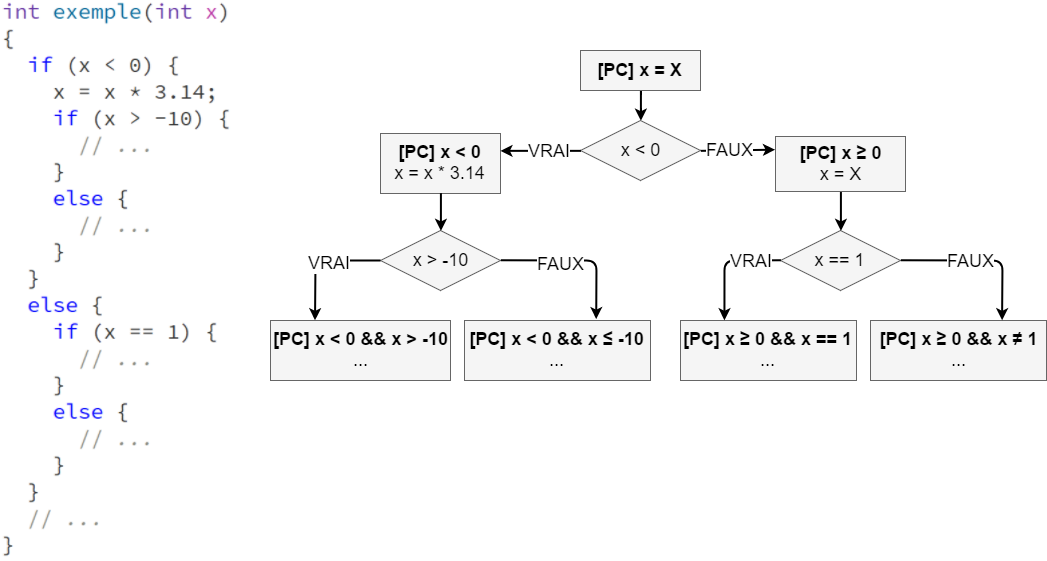
\includegraphics[scale=0.4]{../ressources/images/dynamic_execution_example.png}
    \captionof{figure}{Exemple des chemins d'exécutions possibles récoltés grâce à l'exécution symbolique d'un programme C.}
    \label{symbolic-execution-example1}
\end{center}

%TODO 
%C'est donc une technique qui tire partir des bénéfices des méthodes d'analyses statiques ainsi que des méthodes dynamiques.
%Le problème des méthodes statiques sont les faux positifs et que le programme l'analyse peut potentiellement s'éloigné beaucoup de l'exécution réel du programme.

\subsubsection*{Limitations}
Bien que la technique d'exécution symbolique a été proposée dans les années 70\cite{symbolic-execution-by-king}, cette technique n'a reçu l'attention des chercheurs que récemment pour deux raisons. 
Premièrement l'application de l'exécution symbolique sur des programmes conséquents en application réelle requiert de résoudre des équations complexes avec beaucoup de contraintes. C'est là où les récentes avancées des solveurs de contraintes ont été bénéfiques. Un solveur de contrainte permet de résoudre des équations de satisfaction de contraintes. Il est donc capable d'évaluer la faisabilité d'un ensemble de contraintes donné et permet donc de déterminer si un chemin donné par l'exécution symbolique est faisable ou non. Ces outils sont donc utiliser conjointement à l'exécution symbolique pour limiter l'exécution sur les chemins atteignables.
Deuxièmement, l'exécution symbolique est une technique extrêmement couteuse en ressource, bien plus que les méthodes classiques d'analyse statique. Ce coût est associé à la multiplicité des chemins d'exécution possibles dans des programmes complexes et à la complexité des contraintes des chemins qui augmentent au fur et à mesure du parcours. Heureusement, les puissances de calculs actuelles ont largement augmentées et permettent de réaliser cette analyse dans certaine condition.

Même si l'exécution symbolique semble être théoriquement capable d'analyser en profondeur le comportement d'un programme, cette technique souffre encore de problèmes majeurs quand elle est confronté à de réels programmes:\\
\begin{itemize}
\item Le premier est l'explosion des chemins, c'est à dire que le nombre de chemins d'exécutions possible évolue exponentiellement. Il est donc impératif de trouver des méthodes pour réduire le nombre de chemins à évaluer.\\
\item Le deuxième est la divergence de chemins où \textit{path divergences}. On parle de chemin divergent quand le comportement analysé par l'exécution symbolique est différent du comportement concret à l'exécution. Un tel cas peut arriver plus fréquemment qu'on ne le pense puisque les programmes s'exécutent sur des environnement complexes communicant avec plusieurs composants. L'exécution symbolique ne fait qu'isoler le comportement du programme et il est difficile de tenir compte de tous les éléments pouvant affecter le comportement du programme.\\
\item Le troisième est la complexité des contraintes qui peuvent parfois être trop importantes pour être résolu par un solveur de contraintes. Des contraintes impliquant des opérations de multiplication et de division ou d'autres opérations non linéaires ont tendances à faire rapidement exploser la complexité des contraintes. Si les contraintes de chemins sont indécidables, alors les chemins possiblement couverts par l'exécution symbolique sont limités.

\end{itemize}

%TODO Techniques pour résoudre les problématiques posées plus haut
\subsubsection*{Techniques pour contourner les limitations}
Bien que ces problématiques limitent fortement l'utilisation des techniques d'exécution symbolique sur de réelles applications, il existe des méthodes qui permettent en partie de contourner ces limitations. 
Par exemple, pour contourner le problème d'explosion des chemins, des techniques permettent de guider l'exploration en ce limitant aux chemins amenant à un certain objectif, par exemple celui de couvrir une portion du programme.
Pour limiter la complexité grandissante des contraintes du problème, il est possible de joindre l'exécution symbolique du programme à son exécution concrète, c'est l'exécution concolique. Dans ce cas de figure, le programme est exécuté sur des valeurs concrètes ainsi que sur des valeurs symboliques ce qui permet, si des contraintes deviennent trop complexes, de les simplifier en utilisant les valeurs concrètes du programme. Au final, on se sert de l'exécution du programme pour construire les chemins d'exécutions et de l'exécution symbolique pour limiter le nombre de chemins à exécuter réellement.
%Nous ne souhaitons pas présenter toutes ces méthodes de manière exhaustive puisqu'elles sont nombreuses\cite{orchestrated-survey-automated-test} et certaines de s'appliquent qu'à des cas spécifiques donc nous présenterons une technique pour l'explosion des chemins et une pour la complexité des contraintes. 

\subsection{Model-Based Testing}

\subsubsection*{Définitions}
Model-Based Testing (MBT) est une méthode semi formelle qui utilise des modèles du système testé (\textit{System Under Test: SUT}) pour générer des cas de tests.
Les modèles peuvent représenter des abstractions du comportement du SUT et ils pourront être utilisés pour comparer le comportement théorique modélisé au comportement réel du SUT.
De manière générale, le SUT est modélisé comme une boite noire, c'est à dire que son comportement interne n'est pas analysé. Les modèles décrivent alors des séquences d'entrées et de sorties possibles.
Un des gros avantages de ce type de méthode est qu'elle permet d'abstraire le comportement souhaité du logiciel du code et un modèle pourrait donc définir le comportement souhaité d'un programme, qu'il soit écrit en C ou en Java par exemple.

%Model-based testing (MBT) est une méthode de modélisation semi-formelle dans l'objectif de concevoir de manière automatique ou non des cas de tests. Les modèles peuvent être utilisés pour représenter le comportement voulu du système testé puis pour établir une stratégie de test à partir des modèles.
%
%pour représenter le comportement souhaité du système, pour représenter la stratégie de tests 
%
%est une approche de type ? boîte noire ? c'est
%à dire basée sur la représentation d'un programme sans considérer son fonc-
%tionnement interne. Cette approche vise à identi?er les comportements de
%l'application ou de composants pour véri?er leur comportement en fonction
%des paramètres d'entrées/sorties possibles.
%L'objectif est de trouver un ensemble de valeurs d'entrées pour su?samment tester le comportement du
%programme ou d'une fonctionnalité (couverture de test) à partir, par exemple
%de spéci?cation algébrique [3].

\subsubsection*{Limitations}
Dans notre démarche, nous souhaitons comparer le comportement de programmes dont l'exécution devrait être identique. Nous avons donc une approche qui est orientée à partir du code, c'est à dire que l'objectif des programmes dépend du code source de la programmation qui décrit le comportement souhaité. 
Dans une approche à partir de modèle, l'objectif est souvent inverse. Il est plus facile de décrire les modèles et ensuite de générer une partie du code et des tests. 
Si nous avions décidé d'écrire les exercices de programmation sous forme de modèles, nous aurions pu estimer plus facilement les bénéfices d'une méthode de modélisation. Nous savions qu'une telle approche nécessiterait une compétence technique supplémentaire de l'évaluateur qui devrait être en mesure de décrire le comportement du programme souhaité sous forme de modèle et c'est pour cela que cette méthode n'a pas été privilégiée.
De plus, la quantité d'informations modélisée est souvent limité puisqu'il s'agit de définir principalement le comportement attendu en fonctions des entrées et des sorties. Avec une approche boîte blanche, nous pouvons observer le comportement interne d'un programme et potentiellement découvrir des éléments internes qui favorise l'émergence d'une divergence de comportements entre deux programmes.

%\subsection{Méthodes aléatoires}
%%TODO Y a t-il d'autres méthodes ?
%La génération de test de manière aléatoire est surement une des méthodes
%les plus évidentes et les plus faciles à mettre en place. Dans certains cas, c'est
%l'unique méthode envisageable si la documentation d'un programme est in-
%complète et que le code source n'est pas accessible. Cette technique a bien sur
%un coup important, l'ensemble des valeurs possibles pour les valeurs d'entrées
%d'un programme est souvent trop complexe. Pour cela, des méthodes de gé-
%nération adaptives sont utilisées. Des méthodes empiriques ont montrées que
%des valeurs d'entrées générant des erreurs ont tendance à former des régions
%contingentes d'erreurs. Il en est inversement de même pour des valeurs d'en-
%trées ne générant aucune erreur [2]. Il s'agit donc de dé?nir des stratégies de
%génération pour couvrir de manière e?cace l'ensemble des valeurs possibles
%en maximisant les chances de tomber sur une valeur d'erreur pour ensuite
%tester les valeurs contingentes.

\subsection{Search-Based Testing}
%TODO Search based testing

\subsubsection*{Définitions}
\textit{Search-based software testing}\cite{search-based-testing} est un sous domaine de \textit{Search-based software engineering}\cite{search-based-software-engineering} qui regroupe l'application des heuristiques de recherche pour résoudre des problèmes du génie logiciel.
\textit{Search-based testing}, lui, est le domaine qui regroupe les techniques de recherche heuristique à des fins de générations de tests. Pour cela, il s'agit de transformer le problème de génération de tests en un problème d'optimisation qui peut être résolu avec ces techniques.

Les techniques de recherche heuristiques sont des alternatives pour attaquer les problèmes où l'espace de recherche est trop important. Cette situation est fréquemment rencontrée lorsqu'il s'agit d'établir l'ensemble des chemins d'exécutions possibles d'un programme pour déterminer des jeux de tests pertinents.
L'objectif n'est donc pas de couvrir toutes les branches possibles, mais de définir une fonction objectif qui guidera automatiquement la recherche pour atteindre un but fixé le plus rapidement possible. C'est d'ailleurs le point crucial de cette méthode, puisque c'est cette fonction objectif qui permettra à l'algorithme de déterminer de bonnes solutions dans un temps raisonnable.
Elle peut donc se montrer efficace pour générer des jeux de tests pertinents et pour optimiser le processus de génération de tests.

La forme la plus simple d'un algorithme d'optimisation - bien que très peu efficace - est une recherche aléatoire. Ici, les jeux de tests sont générés aléatoirement jusqu'à ce que l'objectif soit atteint. Un exemple d'objectif simple peut être le pourcentage de couverture du programme à atteindre. Malheureusement cette méthode est très limitée puisque plus l'espace des valeurs possibles est grand moins les valeurs générées aléatoirement auront une chance d'être suffisamment pertinentes.

D'autres techniques sont plus fréquemment utilisées comme celle du \textit{Hill Climbing} qui, appliquée à l'exécution symbolique, favorise la sélection d'optimum locaux. L'algorithme favorise lors de son parcours les chemins les plus prometteurs, c'est à dire que depuis chaque branchement de l'exécution, il sélectionnera le chemin le plus prometteur (par exemple se rapprochant le plus de la solution). Comme un chapitre entier est réservé aux heuristiques, nous ne décrirons pas plus en détail les méthodes de parcours utilisées puisqu'elles sont quasiment identiques.

\begin{center}
    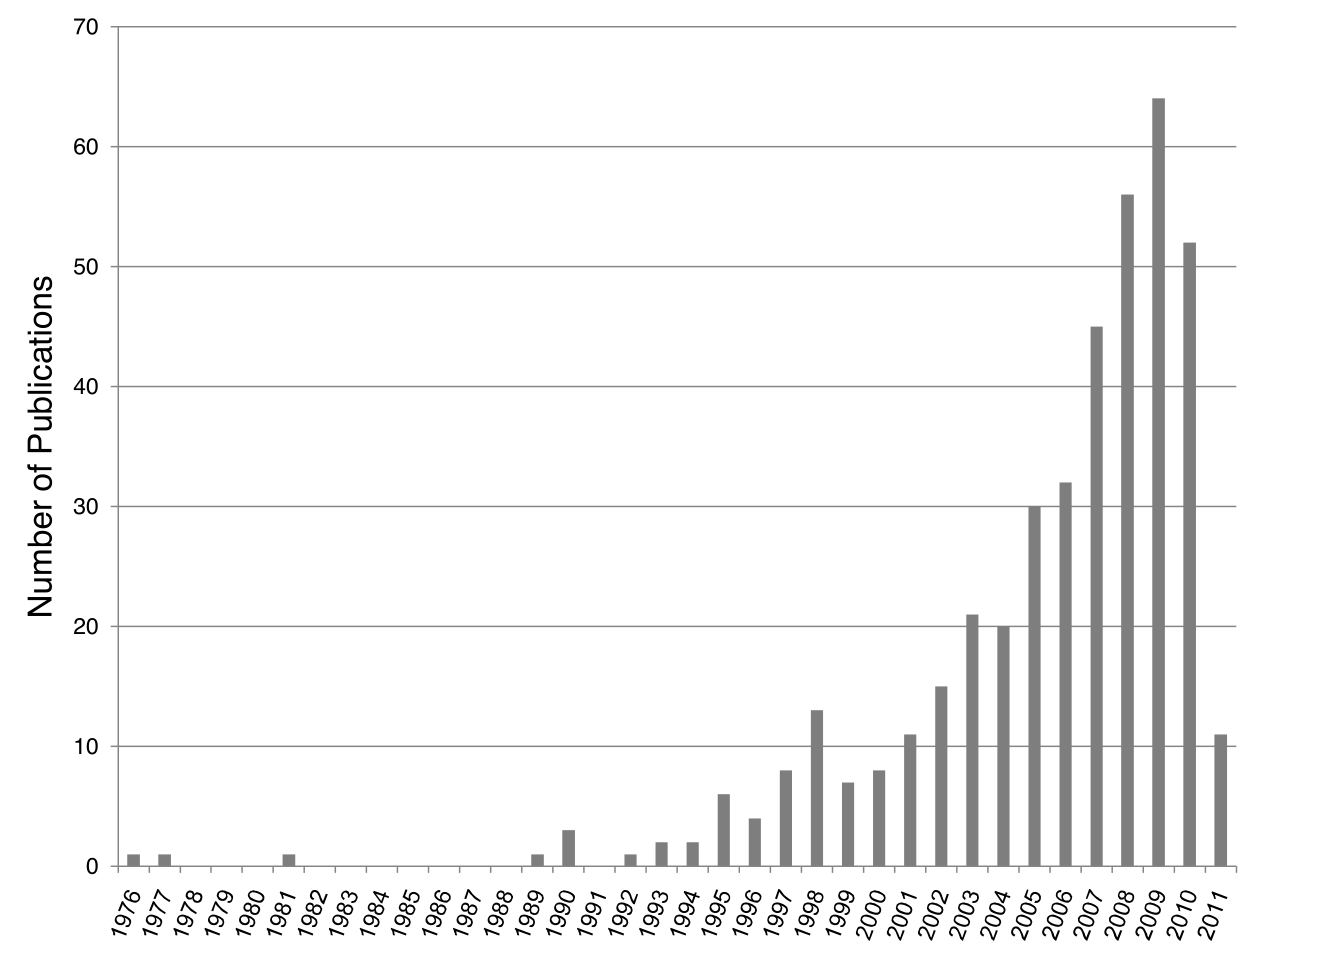
\includegraphics[scale=0.35]{../ressources/images/publications_search_based_testing.png}
    \captionof{figure}{Publications dans le domaine du \textit{Search-Based Software Testing} - source: \textit{Search-Based Software Testing: Past, Present and Future}\cite{search-based-testing}}
    \label{popularity-search-based-testing}
\end{center}


\subsubsection*{Limitations}
Le succès de ces méthodes dépend majoritairement de la qualité de la fonction objectif fixée qui doit permettre de satisfaire un ensemble de critères comme par exemple un pourcentage de couverture des branches à atteindre. De plus, il faut aussi que les outils disponibles puissent tenir compte des critères sélectionnés (le critère peut être indéterminable statiquement ou dynamiquement sur une portion de code) et que l'évaluation de ces critères lors de l'analyse ne soit pas trop longue.

Une fois l'objectif défini, il existe de nombreuses heuristiques de recherche possibles à appliquer. Il faut donc sélectionner la bonne méthode de recherche qui soit apporte un résultat de meilleure qualité, soit le fait en un temps plus raisonnable ou bien les deux à la fois.
Au final, tout le succès de ces méthodes dépend de définition de la fonction objectif qui doit avoir des critères adéquats et déterminables selon la méthode utilisée mais aussi d'une recherche heuristique adaptée au problème qui fasse un compromis entre la qualité de la solution obtenue et le temps d'exécution.

C'est d'ailleurs une limitation importante de ces techniques de recherche puisqu'elles ne sont majoritairement appliquées que pour générer des jeux de tests pour couvrir la plus grand portion du code possible (ou des régions particulière du code ) sans se soucier du comportement de l'application à tester en fonction des valeurs d'entrées.
Heureusement, les méthodes heuristiques permettent d'adapter l'objectif pour qu'il soit pluriel. A l'avenir les défis sont donc de définir des objectifs qui tiennent comptent de multi-critères qui sont déterminables lors de l'analyse et qui permettent de tenir compte du comportement de l'application pour générer des jeux de tests de qualité.

%----------------------------------------------------------------------------------------
%	SECTION 3
%----------------------------------------------------------------------------------------
\section{Détection de divergences entre versions d'un logiciel}

\subsection{Méthode utilisée}
Pour la détection de divergences de comportements entre deux versions d'un même logiciel, il existe des solutions qui permettent de limiter la combinatoire et notamment pour l'exécution symbolique.
Une de ces méthodes proposées est présentée dans l'article \textit{Shadow of a doubt: Testing for divergences Between Software Versions}\cite{shadow} (en référence au célèbre film Alfred Hitchcock: \textit{L'ombre d'un doute}). 

Le postulat de départ est qu'il serait moins coûteux de comparer deux versions d'un même logiciel uniquement aux endroits où le code à été modifié. Au lieu de se baser sur l'analyse complète des deux arbres d'exécution symbolique du programme, nous partirions donc des sous-arbres de ces ensembles, là ou la divergence de code est présente, pour établir l'analyse.
Pour cela, il est proposé de fondre les deux versions du programme en tenant compte des modifications effectuées et ceci grâce à quelques annotations qui permettent de générer des branches d'exécutions séparées là où le code diverge.

%Shadow exemple
\begin{center}
    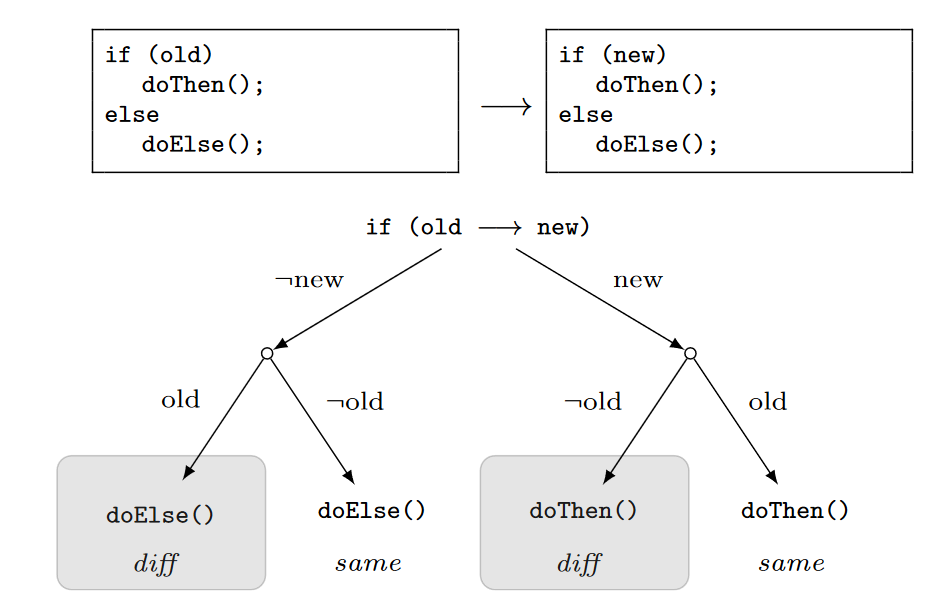
\includegraphics[scale=0.45]{../ressources/images/shadow_example.png}
    \captionof{figure}{Exemple d'un branchemement de l'exécution symbolique tenant compte de la nouvelle version du programme - source: \textit{Article shadow\cite{shadow}}}
    \label{shadow-example}
\end{center}


\subsection{Limitations}
%TODO Il faut le coder, actuellement cette méthode n'est pas automatisée

%Limitation dans notre cas à nous
Même si cette approche paraît particulièrement intéressante, nous doutons de son intérêt dans notre cas où nous ne disposons pas de deux versions d'un même programme mais de n programmes implémentant tous une même spécification (description en langue naturel ou par des formules mathématiques de ce qui doit être produit). 
Potentiellement, ces programmes pourraient être intégralement différents dans leur structure bien que leurs comportements à l'exécution seraient identiques. Il est donc plus difficile de bénéficier de la proximité des programmes pour limiter la combinatoire de l'exécution symbolique.\\

{\setlength{\parindent}{0cm}\textbf{Conclusions:}}

Les approches que nous avons vu précédemment sont souvent limitées\cite{test-auto-solved-yet} de par la complexité grandissante des programmes qui confrontent ces méthodes à l'explosion du nombre de chemins, du nombre d'états ou de contraintes possibles. Pour représenter ces états et chemins, ces méthodes reposent sur des modèles d'arbres qui ne peuvent être parcourus en intégralité à cause de leur taille. Les algorithmes de parcours actuellement utilisés reposent majoritairement sur des stratégies simples comme le parcours en profondeur qui est connu pour être particulièrement couteux mais qui a le bénéfice de trouver au moins un chemin d'exécution possible.

Ces dernières années, grâce à la maturation des recherches sur les différentes stratégies et heuristiques de parcours de graphe (notamment celles avec apprentissage) et des applications récentes sur des problèmes concrets, comme celui du jeu de go où l'ordinateur \textit{AlphaGo}\cite{AlphaGo-research} qui grâce à une implémentation de l'heuristique du Monte Carlo Tree Search a réussi à battre le champion du monde actuel, ces méthodes ce sont popularisées.

C'est pourquoi, nous pensons que des méthodes de Search-based Testing combiner à des méthodes d'exécution symboliques pourraient permettre de contourner nos contraintes. Nous espérons pouvoir utiliser ou simplement nous inspirer des heuristiques avec apprentissages pour diminuer l'espace de recherche plus nous analysons de programme.


%----------------------------------------------------------------------------------------
%	CHAPITRE 2
%----------------------------------------------------------------------------------------
\chapter{Heuristique de recherche} % Nom du premier chapitre

\label{Chapter2} % For referencing the chapter elsewhere, use \ref{Chapter1} 



%----------------------------------------------------------------------------------------
%	SECTION 1
%----------------------------------------------------------------------------------------
\section{Définitions et intérêt}
Les heuristiques sont des critères, méthodes ou principes utilisées pour sélectionner une solution efficace parmi un ensemble possible afin d'atteindre un ou plusieurs objectifs fixés\cite{judea-pearl-heuristics}.
Elles ne sont d'ailleurs pas toujours justes ou fiables dans toutes les situations et peuvent donc être hasardeuses.

Pour une grande majorité des problèmes complexes, déterminer une solution exacte nécessite d'évaluer un immense ensemble de choix. Le temps requis pour trouver cette solution peut être trop important et il est nécessaire parfois de faire des compromis pour obtenir une solution efficace en un temps raisonnable en utilisant une heuristique. 

Elles sont particulièrement utilisées pour répondre aux problèmes dits NP-complet. Ce sont les problèmes pour lesquels tous les algorithmes connus requièrent un temps exponentiel en pire cas pour être résolus. 
Un des exemples les plus connus et fréquemment enseigné en cours d'algorithmique est le problème du voyageur de commerce.

\subsection{Problème du voyageur de commerce (TSP)}
Soit un ensemble de \textit{n} villes réparties et un voyageur souhaitant toutes les parcourir une et une seule fois puis retourner à la ville d'où il est parti et ce en parcourant au total la distance la plus petite possible.

\begin{center}
    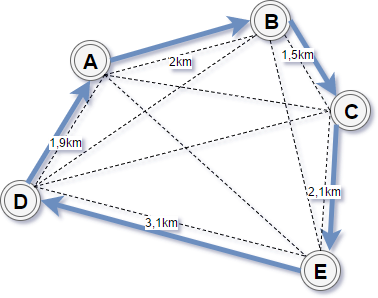
\includegraphics[scale=0.6]{../ressources/images/probleme_voyageur.png}
    \captionof{figure}{Un chemin possible pour résoudre le problème du voyageur de commerce.}
\end{center}

Il existe au total $n!$ chemins possibles soit dans notre cas 120. La ville de départ n'ayant aucune influence sur la longueur totale parcourue on peut donc réduire l'ensemble à $(n-1)!$ soit 24 chemins. Enfin chaque chemin pouvant être parcouru dans les deux sens sans impacter la distance,  on peut donc réduire l'ensemble final à $\frac{1}{2}(n-1)!$ soit 12 chemins.

% Table montrant l'évolution du nombre de chemins en fonction du nombre de villes
\begin{table}[h]
\centering
\begin{tabular}{ l|r }
  Villes & Chemins (solutions) \\
  \hline
  5 & 12 \\
  10 & 181400 \\
  15 & 43 589 145 600 \\
  20 & 60 822 550 204 416 000 \\
\end{tabular}
  \caption{Évolution de l'ensemble des chemins en fonction du nombre de villes pour la résolution du problème du voyageur de commerce}
\end{table}

Le tableau ci-dessus rend compte de la rapidité à laquelle le nombre de chemins à évaluer grandit en fonction du nombre de villes. On parle d'\textit{explosion combinatoire}: c'est le fait qu'un problème se complexifie grandement lorsque le nombre de données à considérer augmente légèrement et peut rendre sa solution incalculable en un temps restreint (longévité humaine par exemple).

\subsection{Un algorithme glouton}
Pour trouver une solution (pas forcément la meilleure) au problème du voyageur de commerce, nous pouvons utiliser une heuristique simple en utilisant un algorithme glouton. Un tel algorithme repose sur le fait de dérouler les données de manière itérative en sélectionnant à chaque étape un optimum local. Ceci a pour effet de grandement diminuer le nombre de données à considérer et donc de répondre en partie à l'explosion combinatoire.

\begin{algorithm}
\caption{Problème du voyageur - un algorithme glouton} 
\label{algo-glouton-TSP}
\begin{algorithmic}
\Function{determiner\_chemin}{$villes, n$}
    \State $P := LISTE\_VIDE$
    \State \textbf{choisir un sommet} u \textbf{dans} villes
    \State $villes := villes - u$
    \State $P := P \cup u$
    \While{$|P| \ne n$}
        \State $d := +\infty$
        \For{v \textbf{in} villes}
            \Comment{Évaluation de la ville la plus proche}
            \If{$distance(u, v) < d$}  
                \State $d := distance(c, v)$
                \State $u` := v$
            \EndIf
        \EndFor
        \State $u := u'$
        \State $P := P \cup u$
        \State $villes := villes - u$
    \EndWhile
    \State \Return $P$
\EndFunction
\end{algorithmic}
\end{algorithm}

L'algorithme \ref{algo-glouton-TSP} présente une heuristique simple pour répondre aux problème d'explosion des chemins en diminuant le nombre de données à évaluer. 
Depuis la ville de départ $u$ (choisit aléatoirement par exemple), il s'agit de sélectionner la ville la plus proche parmi les $n-1$ villes restantes. Puis de manière itérative, nous sélectionnons la prochaine ville la plus proche depuis la dernière ville sélectionnée et ceci jusqu'à ce que toutes les villes soient sélectionnées. 
A la première itération nous avons donc $n-1$ distances à évaluer puis nous en aurons $n-2$ à la deuxième. Au final cet algorithme doit évaluer $\frac{n(n-1)}{2}$ distances. 

\newpage

Ceci montre un exemple simple d'utilisation d'une heuristique qui repose sur la découpe du problème en sous-problèmes pour réduire l'ensemble des données du domaine. L'inconvénient est qu'une telle méthode ne donne pas de garantie de résultât car le chemin le plus court possible n'est retourné que dans le meilleure des cas.
La sélection d'une heuristique pour répondre à un problème réside dans le compromis entre le temps requis pour obtenir une solution et la qualité de la solution retournée c'est à dire sa proximité avec la meilleure solution possible. 
Ces deux critères peuvent être évalués en moyenne, dans le pire cas possible, dans le meilleure cas possible ou bien les trois à la fois. \\

% Table montrant l'évolution du nombre de chemins en fonction du nombre de villes
\begin{table}[h]
\centering
\label{table-comparaison-chemins}
\begin{tabular}{ l|r|r }
  Villes & Chemins & Chemins (algorithme glouton) \\
  \hline
  5  & 12                     & 10  \\
  10 & 18 1400                & 45  \\
  15 & 43 589 145 600         & 105 \\
  20 & 60 822 550 204 416 000 & 190 \\
\end{tabular}
  \caption{Comparaison du nombre de chemins évalués pour la résolution du problème du voyageur de commerce avec un algorithme glouton (heuristique).}
\end{table}

Les heuristiques sont intéressantes en dehors du domaine théorique car la majorité des problèmes pratiques ne nécessite pas d'établir la solution la plus optimale. On préférera trouver un équilibre entre la qualité de la solution obtenue et le coût pour trouver une telle solution qui est un critère non négligeable si l'on prend compte du contexte économique. On parle alors de problème de \textit{semi-optimisation} et plus particulièrement d'optimisation proche lorsque qu'il s'agit de trouver une solution dans un intervalle de coût définie ou de problème d'optimisation approximatif lorsqu'il s'agit de se rapprocher de l'optimum avec une probabilité importante.

%TODO Paragraphe de transition

% SOUS-SECTION 2
\section{Modélisation}
Pour établir une bonne heuristique et évaluer sa capacité à produire des solutions en un temps défini sur un problème donné, il convient de correctement représenter ce problème.
De nombreux problèmes peuvent être formulés comme problème de satisfaction de contraintes - où l'on cherche des états ou des objets satisfaisant un certain nombre de critères - et d'optimisation de tâches. De plus, une heuristique doit pouvoir être automatisée et donc être résolu à l'aide des machines actuels.

Puisque toutes les recherches de solutions à un problème peuvent se résumer à la tâche de construire un object avec les caractéristiques données, les besoins\cite{judea-pearl-heuristics} pour la résolution avec un ordinateur sont les suivants:

\begin{enumerate}
\item Une structure de symbole appelée code ou base de données représentant les sous-ensembles des solutions potentielles.
\item Un ensemble d'opérations ou des règles de production qui modifient les symboles de la base de données pour produire un sous-ensemble de solutions plus fins ou précis.
\item Une procédure de recherche ou stratégie de contrôle qui décide quelles opérations sont à appliquer sur la base de données.
\end{enumerate}

\subsection{Définitions générales}
Les différentes façons de représenter nos problèmes repose majoritairement sur des modèles de graphe. Vous pouvez passer à la section suivante si vous possédez déjà des connaissances de base de théorie des graphes sinon nous décrivons brièvement les notions importantes ici:\\

{\setlength{\parindent}{0cm}\textbf{Graphe:}}

Un graphe est composée d'un ensemble de \textbf{nœuds} ou \textbf{sommets} reliés par des \textbf{arcs} ou \textbf{arêtes} pouvant être associées à des valeurs (par exemple la distance entre deux sommets) ou bien être dirigé (donnant la direction, on va d'un nœud à l'autre).
Dans notre cas, nos graphes auront toujours un nœud de départ appelé \textbf{nœud racine}.
L'ensemble des nœuds est le plus souvent noté $V$ et on note $E$ pour l'ensemble des arêtes du graphe. 
Un graphe est mathématiquement représenté de cette façon: $G = (V, E)$.
Le \textbf{degré} d'un sommet est le nombre d'arêtes de celui-ci.\\

\begin{center}
    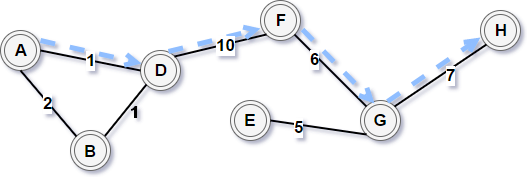
\includegraphics[scale=0.6]{../ressources/images/example_graph.png}
    \captionof{figure}{Représentation d'un graphe à 7 sommets et 7 arêtes avec un chemin dessiné en bleu entre le sommet A et le sommet H: \{A, D, F,G, H\}.}
\end{center}

{\setlength{\parindent}{0cm}\textbf{Arbre:}}

Un arbre est un graphe non orienté dans lequel chaque nœud (sauf le nœud racine) n'a qu'un seul parent. 
On désigne comme \textbf{feuille} un nœud n'ayant aucun fils.
Dans un arbre on définit la \textbf{hauteur} comme étant la longueur du chemin de la racine vers le nœud feuille le plus éloigné. On parle de \textbf{profondeur} quand il s'agit de la distance entre n'importe quel nœud feuille et le nœud racine.
On parle d'\textbf{arbre uniforme} pour désigner un arbre fini de hauteur $n$ dont tous les nœuds qui sont inférieur en profondeur à $n$ ont le même degré et où tous les nœuds de profondeur $n$ sont des feuilles.

\begin{center}
    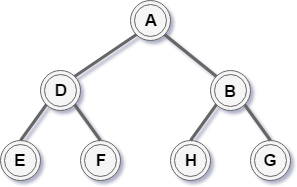
\includegraphics[scale=0.6]{../ressources/images/example_tree.png}
    \captionof{figure}{Un arbre uniforme de profondeur 2 à 7 sommets et 6 arêtes}
\end{center}

%TODO (P.34) Regarder si c'est utile, peut être le déplacer. 
%{\setlength{\parindent}{0cm}\textbf{Recherche dans un graphe:}}
%Dans notre cas, nous recherchons des heuristiques pour répondre à l'explosion combinatoire et donc dans le cas d'une représentation sous forme de graphe nous pouvons aussi parler d'explosion des chemins. L'ensemble des données est parfois tellement importante qu'il est impossible de modéliser l'ensemble.
%Pour combler ces lacunes, il est possible d'utiliser des techniques de génération du graphe pas à pas.

% Beaucoup de problèmes sont décrits comme des tâches pour chercher des propriétés sur un graphe.
% Objectif: Trouver des méthodes efficaces pour trouver la solution rapidement dans le graphe.

Le choix d'une représentation pour encadrer un problème se fait en fonction des contraintes et des données mais ce choix n'est pas unique et peut être différent en fonction de l'approche souhaité.

\subsection{ET-OU graphe}
Le graphe \textit{ET-OU} (ou graphe de réduction de problème) est une modélisation destinée à représenter un problème comme étant la conjonction de plusieurs sous-problèmes qui peuvent être résolus indépendamment.
Cette représentation est principalement utilisée lorsqu'il s'agit de trouver une stratégie de recherche efficace, c'est par exemple le cas si l'on souhaite résoudre le problème de la pièce contrefaite:

Nous avons douze pièces de monnaie et parmi elles se trouve une pièce contrefaite, c'est à dire qui est soit plus légère ou plus lourde que les autres. L'objectif est de déterminer une stratégie pour identifier en au plus trois pesées (avec une balance) quelle est la pièce contrefaite. Il s'agit donc de sélectionner une suite d'actions de ce qui doit être pesé en premier pour avoir une chance d'identifier la pièce contrefaite.
Bien entendu, ce problème peut être résolu en énumérant la totalité des solutions possibles mais l'objectif ici est d'utiliser une heuristique pour identifier une stratégie qui permette de résoudre ce problème en un minimum de pesée (action).

Pour résoudre ce problème, il faut décider du nombre de pièces à comparer à chaque pesée. On peut par exemple décider de peser les pièces une à une, deux à deux, trois à trois, et ainsi de suite. Intuitivement, on sait que si à la première action l'on compare un sous-ensemble de pièces restreint en prenant seulement deux pièces, l'approche sera plus hasardeuse puisqu'à la prochaine action, le sous-ensemble restant risque d'être trop important pour identifier une pièce contrefaite. 
Par contre, si nous pesons deux pièces au hasard en premier, il est possible d'obtenir le résultât en une seule pesée si l'une des deux est soit plus légère ou plus lourde.

Dans ce problème, nous ne sommes pas que confronté au choix de la prochaine action à entreprendre mais aussi aux conséquences de celle-ci qui affecteront inévitablement les prochaines décisions et délimiterons le prochain sous-ensemble.

Pour cela nous utilisons donc le graphe de réduction de problème où les nœuds représentent les sous problèmes et les arcs les conséquences de l'action entreprise sur ce sous-problème. L'avantage de ce type de modélisation est qu'il permet de découper le problème initial en sous-problèmes indépendants grâce à une technique appelée « diviser pour régner ».\\

{\setlength{\parindent}{0cm}\textbf{Arêtes ET:}}

Mène à des sous-problèmes indépendants qui devront tous être résolus pour résoudre le problème associé au nœud père. Cet arc représente les changements dans la situations du problème.\\

{\setlength{\parindent}{0cm}\textbf{Arêtes OU:}}

Mène à des sous-problèmes alternatifs, dont l'un devra être résolu pour résoudre le problème associé au nœud père. Cet arc représente les différentes réactions possible après un tel changement.

\begin{center}
    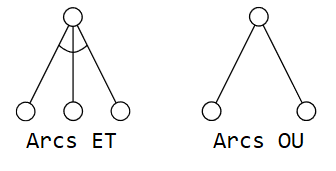
\includegraphics[scale=0.8]{../ressources/images/ET_OU_arcs.png}
    \captionof{figure}{Respectivement les arcs ET et OU du graphe de réduction de problème.}
\end{center}

Nous pouvons donc modéliser notre problème sous forme de graphe où chaque décision prise depuis le nœud racine forme une solution possible résultant de la première action entreprise. Une solution n'est pas donc qu'un chemin dans le graphe, mais un sous-graphe de notre modèle commençant au nœud racine. La figure 1.5 donne un exemple d'une solution possible où l'action de comparer 2 pièces de monnaies est prise en premier.

\begin{center}
    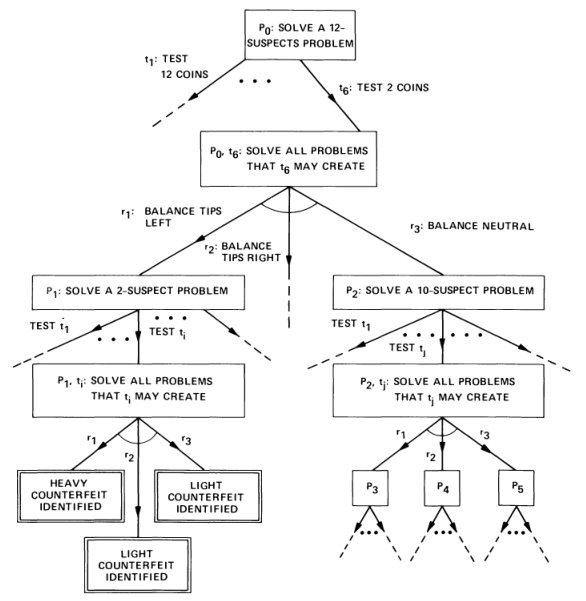
\includegraphics[scale=0.8]{../ressources/images/counterfeit_problem_and_or_graph.png}
    \captionof{figure}{Problème de la pièce contrefaite représenté avec un ET-OU graphe\cite{judea-pearl-heuristics}}
\end{center}

%TODO Conclure + transition

\subsection{Représentation d'état}
Une représentation d'état consiste essentiellement en un ensemble de nœuds représentant chacun les états possibles du problème. Les arêtes entre les nœuds représentent les actions possibles d'un état à un autre. 
Chaque représentation d'état prend la forme d'un graphe ou d'un arbre.

Une représentation sous forme d'espaces états sera plutôt utilisé pour modéliser un problème de satisfaction de contraintes ou de recherche de chemin.
Si la solution peut être exprimée comme une séquence d'actions inconditionnelles ou comme un seul objet avec un ensemble de caractéristiques nous avons un problème de plus court chemin ou de satisfaction de contraintes qui est donc modélisable comme ceci.

Avant de représenter notre problème, il faut préalablement définir un ensemble de facteurs:
\begin{itemize}
\item Quel est l'objectif à atteindre ?
\item Quels sont les actions possibles ?
\item Quels informations doivent être représentées dans la description des états ?
\end{itemize}

Par exemple on peut souhaiter rechercher des erreurs dans un programme. Pour cela, nous pouvons modéliser chaque nœud comme étant un état du programme issu des différentes conditions de branchement où les valeurs concrètes en mémoire seraient remplacées par des valeurs symboliques. Il s'agit alors de parcourir le graphe, pour identifier d'éventuelles valeurs pour lesquelles le programme n'aurait pas le comportement souhaité.

\begin{center}
    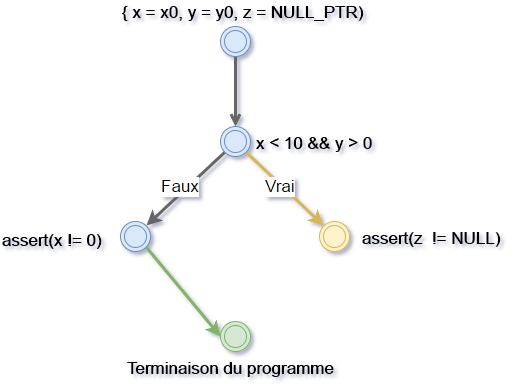
\includegraphics[scale=0.6]{../ressources/images/state_space_graph.png}
    \captionof{figure}{Représentation sous forme d'état de l'exécution symbolique d'un programme}
\end{center}

%TODO (P.34) Définir toutes les notions pour l'explorations des noeuds
%Noeud étendu: Génération de tous les successeurs d'un noeud parant (mais pas les successeurs des successeurs je crois).
%Noeud exploré: Noeud visité
%Noeud généré: Génération d'un noeud successeur à partir de sont parant.
%----------------------------------------------------------------------------------------
%	CHAPITRE 3
%----------------------------------------------------------------------------------------
\chapter{Applications au test logiciel}

\label{Chapter2} % For referencing the chapter elsewhere, use \ref{Chapter2} 

%----------------------------------------------------------------------------------------
%	SECTION 1
%----------------------------------------------------------------------------------------
\section{Le test logiciel}

%----------------------------------------------------------------------------------------
%	SECTION 2
%----------------------------------------------------------------------------------------
\section{Une approche pour la génération automatique de tests}

\subsection{Exécution symbolique}
%TODO 
%Méthode pour simuler l'exécution d'un programme.
%Elle collecte les contraintes des branches de décision et remplace les valeurs des données en mémoire par des valeurs symboliques à base de formules mathématiques.

%----------------------------------------------------------------------------------------
%	SECTION 3
%----------------------------------------------------------------------------------------
\section{État de l'art, tests et heuristiques de recherche}

%\subsection{Article 1}
%TODO
%Path exploration based  on Monte Carlo Tree Search for symbolic execution

%Veut répondre à la problématique de l'explosion des chemins lors du parcours du graphe d'exécution symbolique d'un programme.
%L'article compare les différents algorithme en fonction du nombre de blocs d'instruction parcouru.

%\subsection{Article 2}
%TODO
%Monte Carlo Tree Search for program synthesis
%TODO C'est quoi la synthèse de programme.
%L'objectif de la synthèse de programme est de produire de manière automatique un exécutable d'un segment de code d'un programme qui garantis certains critères.
%Méthode la plus utilisé auparavent: genetic programming.
%----------------------------------------------------------------------------------------
%	Conclusion
%----------------------------------------------------------------------------------------
\chapter*{Conclusion}

\addchaptertocentry{Conclusion}

Dans ce mémoire nous avons présenté les différentes méthodes de génération automatique de tests dont l'exécution symbolique qui nous semblait pouvoir correspondre à notre problème. Même si toutes ces techniques paraissent prometteuses, de nombreuses problématiques ont à chaque fois été rencontrées à cause de la complexité des programmes à analyser (explosion du nombre de chemin, complexité des contraintes, etc.). C'est dans l'optique de trouver des solutions qui nous permettent de générer des tests en un temps raisonnable en utilisant les connaissances récoltées par les analyses précédentes que nous avons décidé de parcourir l'état de l'art des heuristiques de recherche dans l'espoir de comprendre et de pouvoir appliquer une heuristique à une des méthodes de génération pour résoudre notre problème.

Les heuristiques d'apprentissage par renforcement qui se popularisent ces dernières années apparaissent prometteuses pour notre cas d'utilisation. Elles nous permettraient de tirer parti de la variété de nos programmes qui sont supposés exécuter tous un même comportement pour classifier les données et parcourir plus efficacement les arbres d'exécutions associés. C'est pour cette raison que nous nous sommes attardés sur le \textit{Monte Carlo Tree Search} qui permettait de résoudre des problèmes complexes en un temps minimal tout en classifiant les données rencontrées et en proposant des parcours intelligents.

Dans la dernière partie, nous avons présenté une ébauche de méthode pour tirer parti de tous les éléments vu précédemment, c'est à dire de l'exécution symbolique et plus spécifiquement de l'exécution concolique et d'une heuristique inspirée du \textit{Monte Carlo Tree Search}. L'application de cette méthode dans le but de l'évaluer reste problématique puisque les outils d'exécution symbolique sont complexes et qu'il est délicat de les instrumenter dans notre cas d'utilisation pour un initié. De plus, d'autres problématiques se sont posées pour tirer au maximum parti de la classification des données lors de nos parcours. Transposer les données d'un arbre d'exécution symbolique à un autre n'est pas aisé puisque des programmes peuvent appliquer des méthodes différentes pour résoudre un même problème.
Il ne fait aucun doute que le travail à réaliser reste conséquent.


%----------------------------------------------------------------------------------------
%	THESIS CONTENT - APPENDICES
%----------------------------------------------------------------------------------------

% \appendix % Cue to tell LaTeX that the following "chapters" are Appendices

% Include the appendices of the thesis as separate files from the Appendices folder
% Uncomment the lines as you write the Appendices

% % Appendix A

\chapter{Frequently Asked Questions} % Main appendix title

\label{AppendixA} % For referencing this appendix elsewhere, use \ref{AppendixA}

\section{How do I change the colors of links?}

The color of links can be changed to your liking using:

{\small\verb!\hypersetup{urlcolor=red}!}, or

{\small\verb!\hypersetup{citecolor=green}!}, or

{\small\verb!\hypersetup{allcolor=blue}!}.

\noindent If you want to completely hide the links, you can use:

{\small\verb!\hypersetup{allcolors=.}!}, or even better: 

{\small\verb!\hypersetup{hidelinks}!}.

\noindent If you want to have obvious links in the PDF but not the printed text, use:

{\small\verb!\hypersetup{colorlinks=false}!}.

% \include{Appendices/AppendixB}
% \include{Appendices/AppendixC}

%----------------------------------------------------------------------------------------
%	BIBLIOGRAPHY
%----------------------------------------------------------------------------------------

\printbibliography[heading=bibintoc]

%----------------------------------------------------------------------------------------

\end{document}  
